\documentclass{article}
\title{ECE 370 -- Homework 1}
\usepackage{graphicx}
\usepackage{pdfpages}
\usepackage{fancyhdr}
\usepackage{enumitem}
\usepackage{amsmath}
\pagestyle{fancy}
\fancyhf{}
\fancyhead[L]{Gianni Avilan-Losee}
\fancyhead[C]{ECE 370}
\fancyhead[R]{Homework 1}
\fancyfoot[C]{\thepage}
\usepackage{microtype}
\usepackage{textcomp, gensymb}
\author{Gianni Avilan-Losee}
\setcounter{section}{1}
\begin{document}
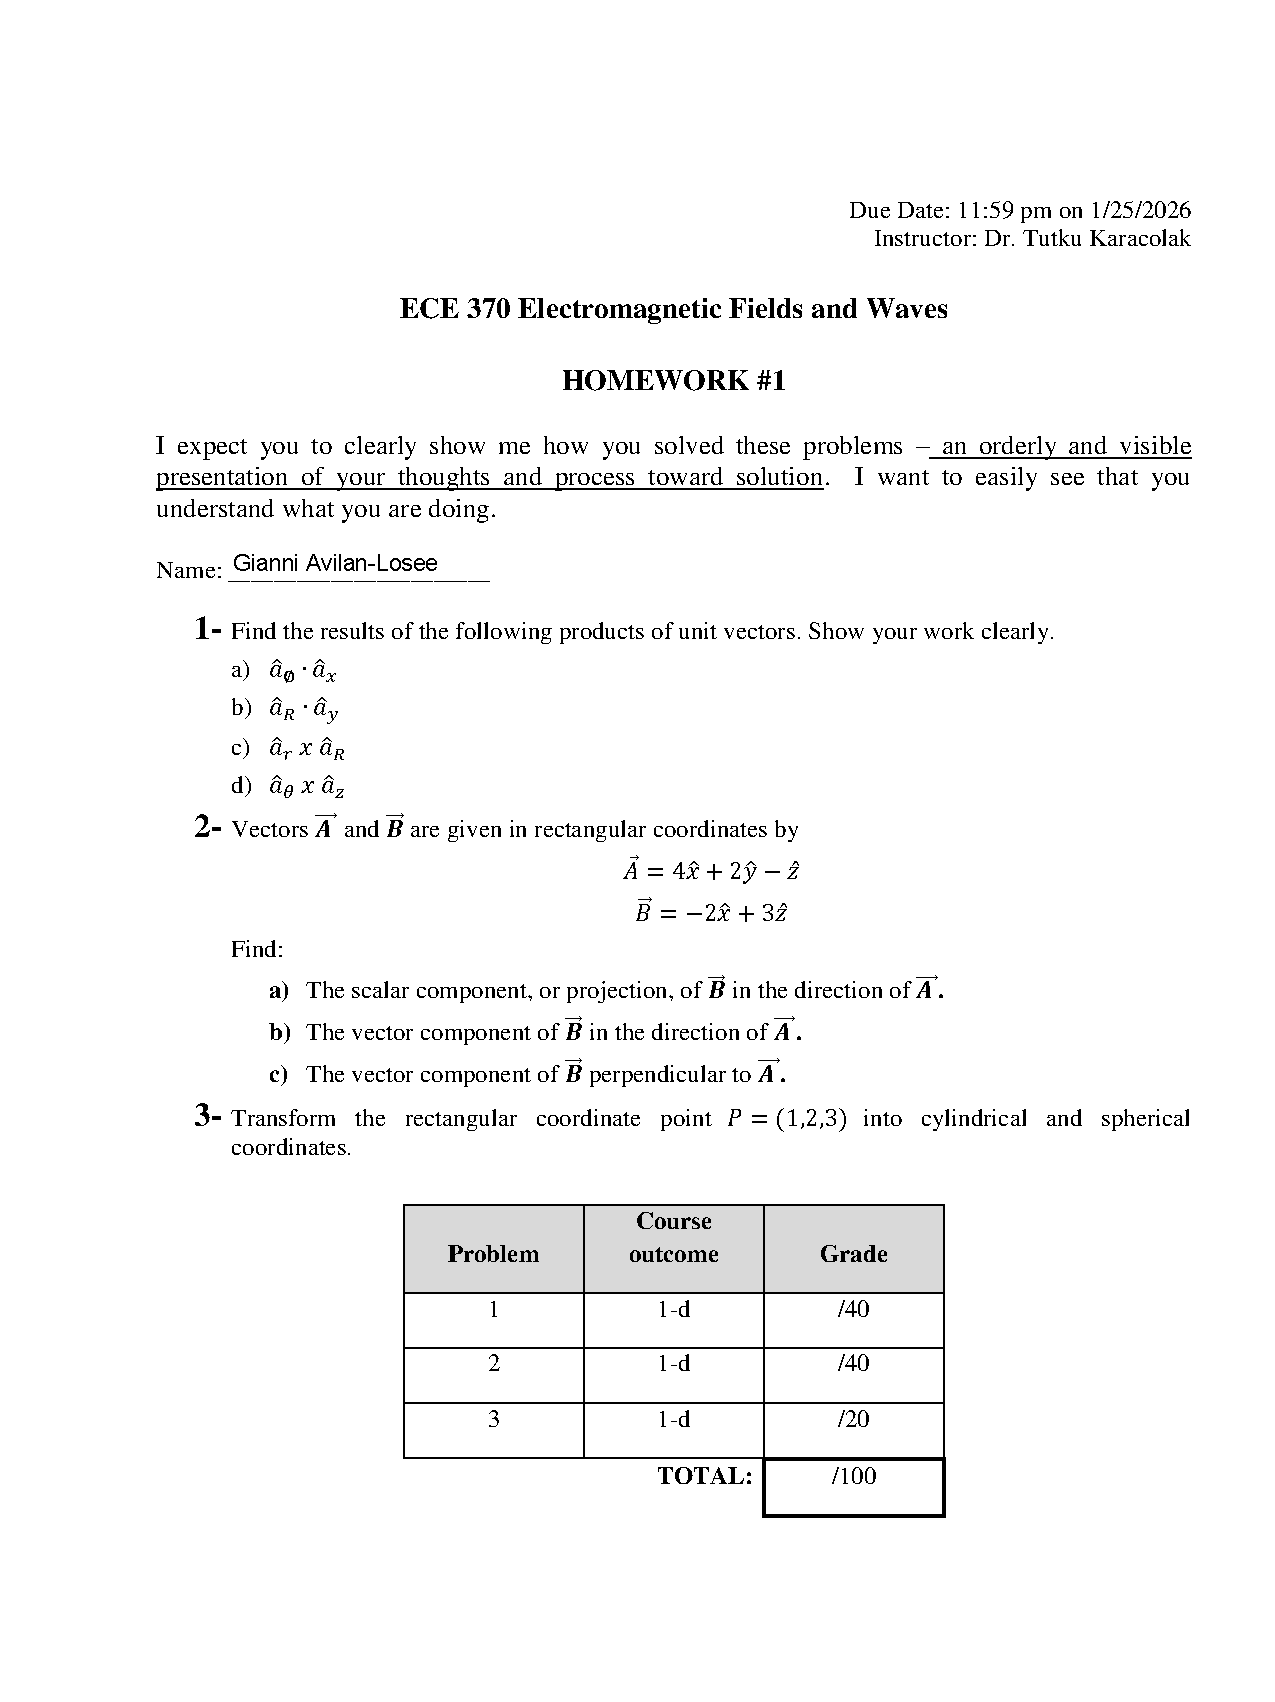
\includepdf{homework-1_cover-page.pdf}
\begin{enumerate}
	\item
\begin{enumerate}[label=\alph*)]
	\item In the cylindrical coordinate system, $\hat{\alpha_r}$'s direction is a function of the angle $\phi$, as measured counterclockwise from the positive x-axis, and restricted to the range $0 \leq \phi < 2\pi$. In summary, we may assume an angle \(\phi\) between \(\hat{\alpha_x}\) and \(\hat{\alpha_r}\).

	Next, we may assume an angle of $90\degree$ between $\hat{\alpha_r}$ and $\hat{\alpha_{\phi}}$, since all basis vectors in the cylindrical coordinate system are orthogonal, and so define the angle between $\hat{\alpha_x}$ and $\hat{\alpha_{\phi}}$ as $\phi + 90\degree$. By the definition of the dot product, $\hat{\alpha_\phi} \cdot \hat{\alpha_{x}} = |\hat{\alpha_{\phi}}| \space |\hat{\alpha_{x}}|cos(\theta_{\hat{\alpha_{\phi}}\hat{\alpha_{r}}})$, where $\theta_{\hat{\alpha_{\phi}}\hat{\alpha_{r}}}$ is the angle between the two vectors. Since the magnitude of both vectors $|\hat{\alpha_{r}}|=|\hat{\alpha_{\phi}}| = 1$, $$\hat{\alpha_{\phi}} \cdot \hat{\alpha_r} = cos(\theta_{\hat{\alpha_{\phi}}\hat{\alpha_{r}}})=cos(\phi + 90\degree) = -sin(\phi).$$ We can double check this result by using the coordinate system transforms given in Table 3-2 of the textbook, where $\hat{\alpha_x} = \hat{\alpha_r}cos(\phi) - \hat{\alpha_{\phi}}sin(\phi)$; and so, keeping in mind that the dot product is distributive, $$\hat{\alpha_{\phi}} \cdot \hat{\alpha_x} = \hat{\alpha_{\phi}} \cdot (\hat{\alpha_r}cos(\phi) - \hat{\alpha_{\phi}}sin(\phi)) = \hat{\alpha_{\phi}} \cdot \hat{\alpha_r}cos(\phi) - \hat{\alpha_{\phi}} \cdot \hat{\alpha_{\phi}}sin(\phi).$$ Note that multiplying either unit vector by a scalar does not affect the angular relationship between it and another vector. Since $\hat{\alpha_{\phi}}$ and $\hat{\alpha_r}$ are orthogonal, their dot product is equal to $0$, while the dot product between the identical vectors $\hat{\alpha_{\phi}}$ is equal to $1$. Thus, the dot product simplifies to $$\hat{\alpha_{\phi}} \cdot \hat{\alpha_r} = -sin(\phi).$$

  \item $\hat{\alpha_{R}}$'s direction is a function of both the zenith angle $\theta$ and the azimuth angle $\phi$, similar to how $\hat{\alpha}_r$ is determined relative to $\phi$ in the cylindrical coordinate system. In this case, we can locate the unit vector $\hat{\alpha_R}$ at an angle $\theta$ from the positive z-axis and an angle $\phi$ from the positive x-axis in the rectangular system. 

  Transforming \(\hat{\alpha_R}\) into the rectangular coordinate system, \[
		\hat{\alpha_R} = \hat{\alpha_x}sin(\theta)cos(\phi) + \hat{\alpha_y}sin(\theta)sin(\phi) + \hat{\alpha_z}cos(\theta).
	\]
	Once again applying the distributive property of the dot product and reducing orthogonal vectors to zero, as in question 1a, we are left with \[
	 \hat{\alpha_R} \cdot \hat{\alpha_y} = sin(\theta)sin(\phi). 
	\]	

	\item First, defining any cross product \(\vec{A} \times \vec{B} = |A|\space|B|sin(\theta_{AB})\hat{n}\), where \(\hat{n}\) is the unit normal vector, whose direction is found using the right hand rule, we assume as before that, since \(\hat{\alpha_{r}}\) and \(\hat{\alpha_{R}}\) are unit vectors and have a magnitude of 1, their cross product simplifies to \(\hat{\alpha_{r}} \times \hat{\alpha_{R}} = sin(\theta_{AB})\hat{n}\). 

		The cross product \(\vec{A} \times \vec{B}\) may also be expressed in the form of a determinant (in cylindrical coordinates), as \[
			\vec{A} \times \vec{B} = \begin{vmatrix}
				\hat{\alpha_r} & \hat{\alpha_{\phi}} & \hat{\alpha_z} \\
				A_r & A_{\phi} & A_z \\
				B_r & B_{\phi} & B_z
			\end{vmatrix}
		\] 
	Transforming the unit vector of \(\hat{\alpha_R} = \hat{\alpha_r}sin(\theta) + \hat{\alpha_z}cos(\theta)\), we may express the cross product between the two given unit vectors as \[
	  \hat{\alpha_r} \times \hat{\alpha_r} = \hat{\alpha_r} \times \hat{\alpha_r}sin(\theta) + \hat{\alpha_r} \times \hat{\alpha_z}cos(\theta).
  \] 
	Assuming that the cross product between the identical vectors \(\hat{\alpha_r}\) equals zero, irrespective of either vector's scaling, we may then express the cross product in determinant form as \[
		\hat{\alpha_r} \times \hat{\alpha_z}cos(\theta) = \begin{vmatrix}
			\hat{\alpha_r} & \hat{\alpha_{\phi}} & \hat{\alpha_z} \\
			A_r & A_{\phi} & A_z \\
			B_rcos(\theta) & B_{\phi}cos(\theta) & B_zcos(\theta)
		\end{vmatrix}.
	\]
	Since both quantities are unit vectors, the entire determinant simplifies to \(-\hat{\alpha_{\phi}}cos(\theta)\). Therefore, \[
		\hat{\alpha_r} \times \hat{\alpha_R} = -\hat{\alpha_{\phi}}cos(\theta).
	\]
	This concurs with the use of the right-hand rule, which indicates that any cross-product between the two unit vectors should be orthogonal to the \(\phi\)-\(z\) plane, depending on the order in which the cross product is taken.

  \item In this case, we may transform \(\hat{\alpha_{\theta}}\) into its cylindrical components as \(\hat{\alpha_{\theta}}=\hat{\alpha_r}cos(\theta) - \hat{\alpha_z}sin(\theta)\), which expands the given cross product to \[
		\hat{\alpha_r}cos\theta - \hat{\alpha_z}sin(\theta) \times \hat{\alpha_z}. 
\]
	Making use of the anti-commutative and distributive properties of the cross product, this may be further simplified to \[
		-[\hat{\alpha_z} \times \hat{\alpha_r}cos(\theta) + \hat{\alpha_z} \times \hat{\alpha_z}sin(\theta)] = \hat{\alpha_z} \times \hat{\alpha_r}cos(\theta). 
	\]
	Using the determinant definition of the dot product as before,\[
		\hat{\alpha_z} \times \hat{\alpha_z}cos(\theta)=\begin{vmatrix}
			\hat{\alpha_r} & \hat{\alpha_{\phi}} & \hat{\alpha_z} \\
			0 & 0 & -1 \\
			cos(\theta) & 0 & 0 
		\end{vmatrix} = -\hat{\alpha_{\phi}}cos(\theta),
	\]
	which also corresponds with the directional component given by the right-hand rule. 

\end{enumerate}
\item 
\begin{enumerate}[label=\alph*)]
	\item The scalar component of \(\vec{B}\) in the direction of \(\vec{A}\) is found by means of the dot product between \(\vec{B}\) and the unit vector pointing in the direction of \(\vec{A}\). First, finding the unit vector pointing in the direction of \(\vec{A}\), \[
			\hat{\alpha_A} = \frac{\vec{A}}{|\vec{A}|} = \hat{\alpha_x}\frac{4}{\sqrt{21}} + \hat{\alpha_y}\frac{2}{\sqrt{21}} - \hat{\alpha_z}\frac{1}{\sqrt{21}}.	
	\]
	Then, the scalar component of \(\vec{B}\) in the direction of \(\vec{A}\) is \[
		\vec{B} \cdot \hat{\alpha_A} = \frac{-8}{\sqrt{21}} - \frac{3}{\sqrt{21}}=-\frac{11}{\sqrt{21}}.
	\]
  \item To find the vector component or projection of \(\vec{B}\) in the direction  of \(\vec{A}\), we must find the vector whose magnitude is the scalar projection of \(\vec{B}\) on \(\vec{A}\) with the same direction of \(\vec{A}\).
		To find this, we may simply scale the unit vector pointing in the \(\vec{A}\) direction by the scalar component of \(\vec{B}\) in the \(\vec{A}\) direction, \[
			(\vec{B} \cdot \hat{\alpha_A})\hat{\alpha_A}=-\hat{\alpha_x}\frac{44}{21} - \hat{\alpha_y}\frac{22}{21}+\hat{\alpha_z}\frac{11}{21}.
		\] 
	\item Finally, to find the vector component of \(\vec{B}\) in the direction of \(A\), we may use the property that the sum of \(\vec{B}\)'s vector component parallel to and perpendicular to the direction of \(A\) will equal \(\vec{B}\). In other words, \(\vec{B}\) is made up of a component parallel to the \(\vec{A}\) direction and another component orthogonal to the \(\vec{A}\) direction. Therefore, the component orthogonal to the \(\vec{A}\) direction is given by \[
			\vec{B} - [(\vec{B} \cdot \hat{\alpha_A})\hat{\alpha_A}] = \hat{\alpha_x}\frac{2}{21} + \hat{\alpha_y}\frac{22}{21} + \hat{\alpha_z}\frac{52}{21}. 
	\]
\end{enumerate}
\item Given the point \(P(1,2,3)\) in rectangular coordinates, we may first convert \(P\) to cylindrical coordinates of the form \(P(r,\phi, z)\) by using the coordinate transformations \(r=\sqrt[+]{x^2+y^2}, \space\phi = atan2(\frac{y}{x})\), and \(z=z\). Therefore, \[
		P_{rectangular}(1,2,3) = P_{cylindrical}(2.236, 63.43\degree, 3).
\]
Converting to spherical coordinates, we may use the coordinate transformations \(R = \sqrt[+]{x^2+y^2+z^2}, \space \theta = atan2(\frac{\sqrt[+]{x^2+y^2}}{z}),\) and \(\phi = atan2(\frac{y}{x})\). Therefore, \[
	P_{rectangular}(1,2,3) = P_{cylindrical}(3.7417, 36.70\degree, 63.43\degree).
\]
\end{enumerate}
\end{document} 
